\chapter{Methodology}\label{chap:Methodology}
\subsubsection{Single-cell RNA-sequencing Dataset}
The scRNA-seq dataset used in this project was generated by Ana Veloso from the Zinzen lab, MDC-BIMSB, 
and was pre-processed by Yozlem Bahar from the Wolf lab in MDC. 
The dataset was generated using 10X Genomics approach, by a protocol developed by Veloso (2022) to specifically 
target NBs cells of the Drosophila embryos in the sequencing. 
The dataset contains samples from two partially overlapping time points that span developmental stages 8 to mid-stage 10, 
in which the NBs delamination waves S1-S3 take place.

The dataset underwent both cell-level and gene-level filtering by Bahar. 
Additionally, Bahar annotated the dataset for NBs cell types by clustering and identifying marker genes. 
For further details, see Bahar (2024).

\section{GRN inference from scRNA-seq Dataset} 
\subsubsection{SCENIC workflow}
A GRN was infered from the dataset using pySCENIC 
(Van de Sande et al., 2020 \cite{van2020scalable}) v.0.12.1, a Python implementation of the SCENIC workflow, 
available as a Python package. 
A Python script was written to run the SCENIC workflow.
The full script will be made publicly available in Github - add link here. 
The script utilizes the three main steps of SCENIC in a pipeline manner, where the output of one step is the input of the next.

Here, the SCENIC workflow used the \textit{GRNBoost2} \cite{moerman2019grnboost2} method for the initial co-expression 
modules construction, followed by the motif enrichment (\textit{i-cisTarget}) and cellular enrichment (\textit{AUCell}) steps, 
called here also the first, second and third step respectively. 

\subsubsection{Additional input used in the SCENIC workflow}
SCENIC workflow was run sequentially where one step's output is the input for the next one. 
The first step requires a gene expression matrix, which here is the counts matrix of the pre-processed dataset 
(without any annotations, like cell types). 
Additionally, SCENIC incorporates input from databases for the first and second step, as follows:

\begin{itemize}
    \item \textbf{Step 1:} co-expression modules construction (GRNBoost2)
    \begin{itemize}
        \item \textbf{Species specific list of candidate TFs} A list of all known TFs in Drosophila
    \end{itemize}
   \item \textbf{Step 2:} Motif enrichment (i-cisTarget)
   \begin{itemize}
       \item \textbf{Motif ranking database} Drosophila Whole genome rankings for regulatory motifs
       \item \textbf{Motif Annotations database} Drosophila regulatory motifs annotations
   \end{itemize}
\end{itemize}

The databases were sourced from the Stein Aerts Lab website (\url{https://resources.aertslab.org/cistarget} ), 
which utilises data from FlyBase \cite{thurmond2019flybase}, a database for Drosophila genetics and molecular biology, 
along with databases related to other species. When not available, one can create custom databases suitable for SCENIC 
(see \url{https://scenic.aertslab.org}).

\subsubsection{Multiple iterations}
As described in the background section, GRNBoost2 is stochastic, which means that every time the workflow is run, 
the inferred GRN is somewhat different. To address this variability, the workflow was executed 50 times, following the 
recommendation of Van de Sande et al. (2020)  \cite{van2020scalable}. As illustrated in fig. \ref{fig:workflow_diagram}, 
regulons that appear in more than 80\% of the runs (> 40 runs) were considered for further analysis of the GRN. In more detail, 
a list of regulons is produced after the motif enrichment step in the SCENIC workflow, and each each regulon consists of a 
TF and an accompanying list of target genes. TFs (the head of regulons)  were aggregated across runs, and those appearing 
in over 40 runs were saved as a subset for further analysis.
For convenience purposes, the persistent regulons that were common for over 80\% of the iterations will be referred to as 
\textit{core regulons.}

\begin{figure}
    \centering
    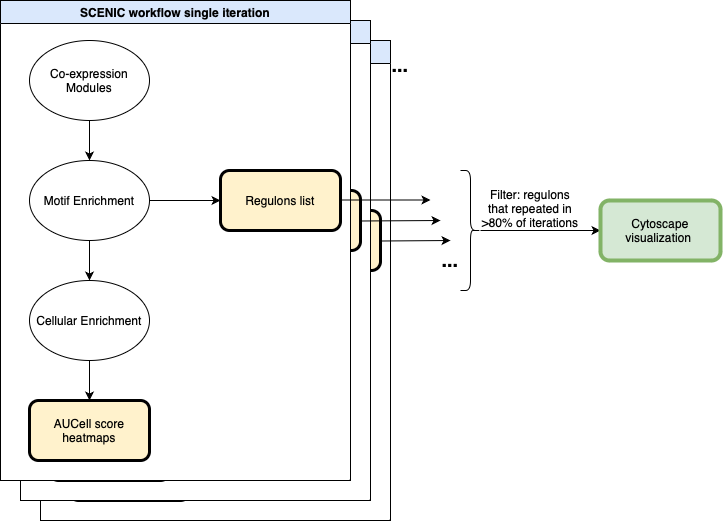
\includegraphics[scale=0.5]{figures/methods/workflow_diagram.png}
    \caption{Illustration for multiple iterations of SCENIC workflow}
    \label{fig:workflow_diagram}
\end{figure}

\subsubsection{Cellular enrichment clustering and visualisation in heatmaps}
The third and last step of SCENIC is cellular enrichment, in which each regulon gets an AUCell score that symbolises its 
activity in each of the cells in the dataset. 
In each SCENIC iteration, a matrix of $cells \times regulons$ is produced, with the AUCell scores. 
This matrix was clustered and visualized in a heatmap using Python's $seaborn.clustermap$ hierarchical clustering method.
Additionally, cell types annotations of the dataset were added to the heatmap.

From this AUCell score heatmap .. more heatmaps were produced:

\begin{itemize}
    \item \textbf{Binary heatmaps:} to binarize the AUCell score, a two-component Gaussian mixture model is fitted to define 
        a threshold. This threshold labels cells as 'on' or 'off' for each regulon. When the AUCell distribution across cells 
        is skewed, the threshold is set along the right tail of the distribution \cite{van2020scalable}. 
        Thresholds can be tuned or set manually according to biological knowledge, however here the binarization was not 
        manually changed, due to lack of biological knowledge.
    \item Reduced heatmap for the persistent regulons
    \item AUCell score heatmap grouped by average AUCell score per cell type. 
\end{itemize}



\section{GRN Visualization}
The SCENIC-inferred GRN is inferred after the motif enrichment step of SCENIC. The subset of regulons that repeated across  
over 40 runs were extracted and exported as a CSV file containing TF-target genes pairs, and their occurrence count across runs. 
This CSV was visualized as a network using Cytoscape software (Shannon et al., 2003 \cite{shannon2003cytoscape}) 
v.3.10.0. The network was contains TFs and target genes as nodes, with directional edges from a TF to its target genes. 
Some TFs are also target genes of other TFs. TFs and target genes were styled differently for better readability by uploading 
an additional list of annotations of genes as TFs or target genes. 
Within Cytoscape, the count of reoccurring TF-target gene across iterations was captured as the thickness of the regulatory edges. 
Thicker edge shows higher occurrence across SCENIC iterations. 
The GRN was then filtered to show the known marker genes of NBs, and their nearest neighbors.

\
\section{Boolean Model Analysis}
\subsubsection{Boolean model of signaling mechanism if early Drosophila nervous system development}
A Boolean model of the signaling mechanism in Drosophila during early development, that was developed by Yozlem Bahar from the 
Wolf lab at MDC, was analysed here. Fig. \ref{fig:BoolModel1} illustrates its topography. The model consists of 30 nodes and 57 
directed edges. Nodes represent genes and edges represent a regulatory relationship of transcription activation (green edges) 
or suppression (red edges). This model is based on literature knowledge about signalling pathways, and marker genes that 
characterize different NBs types. 
The yellow nodes are input nodes that represent signaling pathways, namely Hh, Wg and Egfr. Gray nodes represent marker genes. 
Round nodes represent NB cell types.  Six NBs types are included in this model, namely 5-6, 5-3, 5-2, 6-2, 7-4, 7-1. 
The model with the full logical rules is available in the supplementary materials. 

\begin{figure}[ht]
    \centering
    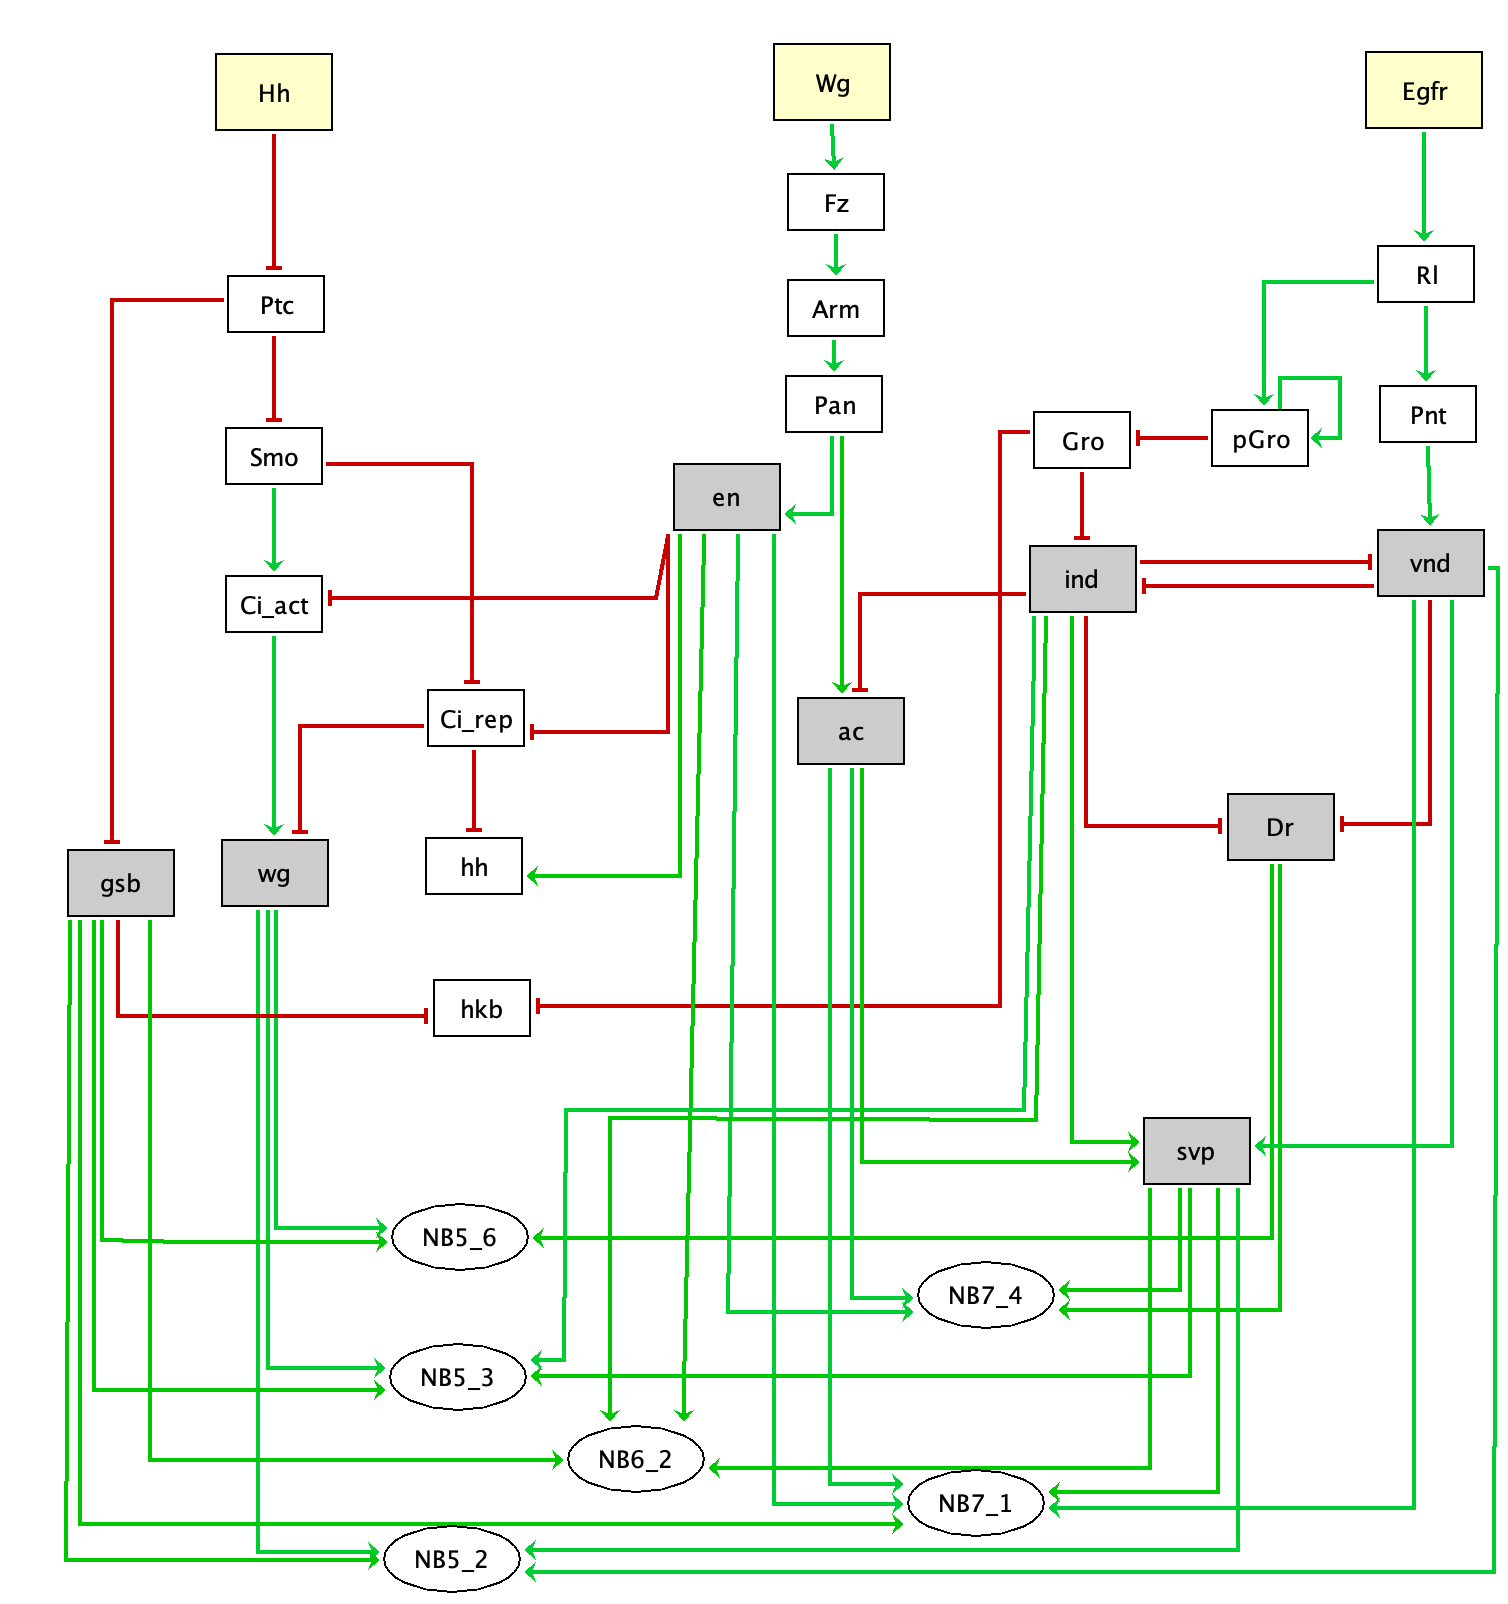
\includegraphics[scale=0.5]{figures/methods/Original_Model.png}
    \caption{Boolean model of Drosophila GRN during neuroblasts specification. Developed by Yozlem Bahar, Wolf lab, MDC (2024)}
    
    \label{fig:BoolModel1}
\end{figure}

\subsection{Stable state analysis}
Gene Interaction Network simulation (GINsim), Gonzalez et al. (2006)\cite{gonzalez2006ginsim} is a software designed to edit, 
simulate and analyse logical models of regulatory networks.
Here, GINsim v.3.0 \cite{naldi2018logical} was used to calculate the stable states, or fixed points, of the Boolean model in 
both the graphic user interface and as a python package, available via CoLoMoTo \cite{naldi2018colomoto}, a Python interface 
developed for various tools for the construction and analysis of logical models. 
Stable states were calculated in GINsim to reproduce to the stable states analysis done by Bahar et al. 

\subsubsection{Correlation of Variables}
Stable states tables were further analysed by calculating the pairwise correlation between the different variables. 
Kendall rank correlation was used.  

\subsubsection{Perturbation Analysis}
Knock out perturbation was done by iteratively setting one node at a time to 0, and calculating the stable states with 
that perturbation. 

\section{Boolean Model Extension with GRN Inferred from Single Cell Sequencing Data}
The Boolean model was compared to the GRN filtered in different ways, as will be shown in the results 
(section \ref{chap:results}). 
The GRN in Cytoscape filtered to contain the marker genes, which appear in the Boolean model, and their direct neighbors, 
was compared to the model. New regulatory relationships that include nodes or edges that did not appear in the model 
but are connected directly according to the SCENIC GRN, were searched for validation in literature and in FlyBase database. 
New nodes and edges with defined logical rules were added to the Boolean model based on literature.
The extended model underwent stable state analysis and compared to the original model. 
 


